% Generated from the closed, failed component campaign by make_components.py.
\subsection{Prepared-input component controls: qualification failures}
\label{app:seg-laptop-components}
Following the accepted total-pipeline sessions, a separate prospective protocol fixes two prepared-input endpoints on the same laptop and frozen image pairs: blocks of 64 original torchvision NMS calls on captured boxes/scores, and one native mask-renderer call on cached prototypes and retained detections. NMS per-call estimates divide whole-block timing by 64 and include the Python facade/loop/index release; mask output release occurs after timing. Preparation is outside timing. These different cache and lifetime scopes are not an additive decomposition of the earlier pipeline.
The NMS two-image smoke completes 384 trials with zero of four reference blocks flagged, permitting one 20-image full run. The full run completes all 3840 trials and all input-immutability, prediction/count, affinity and source audits, but fails its registered reference-drift criterion: 20 of 22 blocks are flagged (maximum allowed: two). Nineteen flagged references are faster than the initial reference and one is slower. Therefore this failure cannot be described simply as progressive slowing; the physical cause is unresolved.
The full NMS duplicate-label A/A MDEs are 0.340730\% (clean) and 0.095851\% (attacked). Passing these two precision bounds does not override the failed reference gate.
The distinct, predetermined native-mask smoke completes 384 trials but flags its final reference (ratio 1.0328367896175703), exceeding the smoke allowance of zero flags. Its full run is cancelled. No component is repeated, no gate is relaxed, and neither contrast is eligible for primary inference. Testing placeholders of one preserve the declared two-comparison family but are not evidence of no effect. Apparent component ratios remain in diagnostic artifacts only.
\begin{figure*}[t]\centering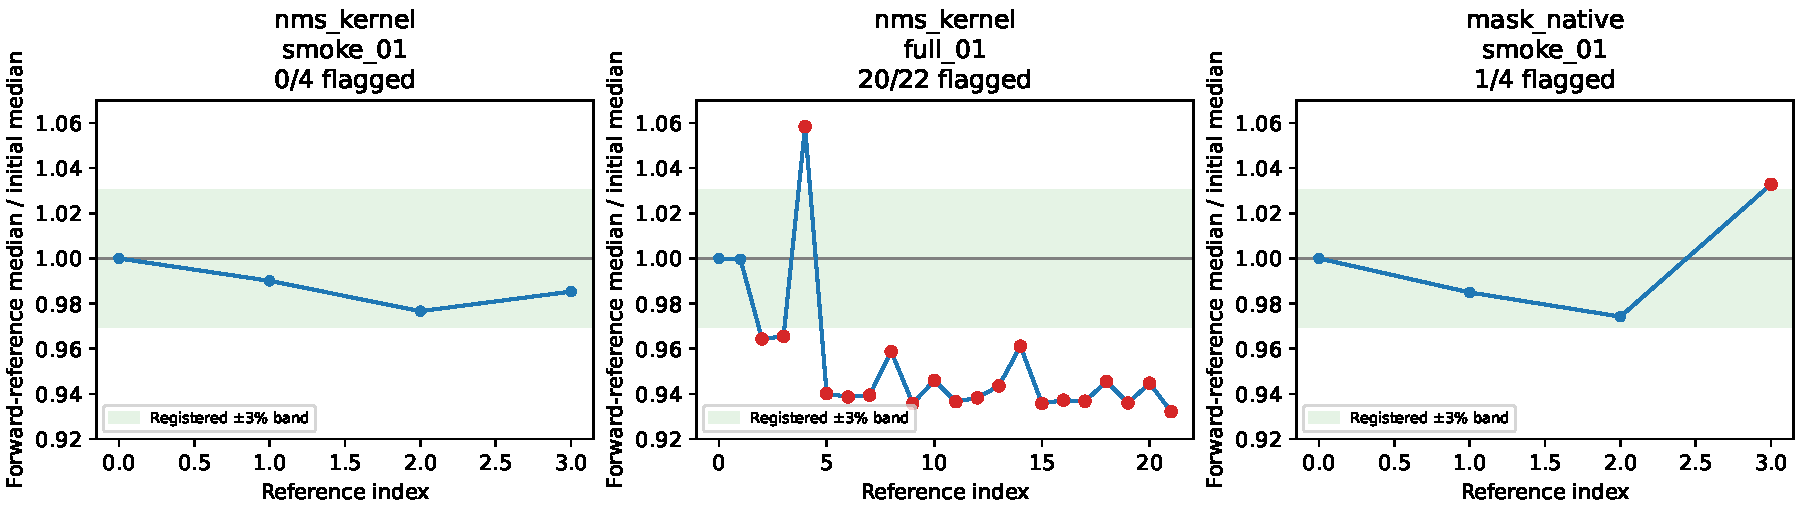
\includegraphics[width=.98\textwidth]{segmentation_extension/laptop_components.pdf}\caption{All reference blocks in the closed component campaign. Shading marks the registered 3\% band; red points are flagged. Both full component contrasts remain unqualified.}\label{fig:seg-laptop-components}\end{figure*}
All three completed runs restore the original affinity of 45 application processes. Failed component controls do not invalidate separately qualified total-pipeline or paired-defense sessions, and do not supply additional evidence of service denial, tail stability, physical attacks or ARM performance.
